% !TeX root = ./2019-20-COMP360-05-workshop-materials_screen.tex
% Adjust these for the path of the theme and its graphics, relative to this file
%\usepackage{beamerthemeFalmouthGamesAcademy}
\usepackage{../../beamerthemeFalmouthGamesAcademy}
\usepackage{multimedia}
\graphicspath{ {../../} }

% Default language for code listings
\lstset{language=C++,
        morekeywords={each,in,nullptr}
}

% For strikethrough effect
\usepackage[normalem]{ulem}
\usepackage{wasysym}

\usepackage{pdfpages}

% http://www.texample.net/tikz/examples/state-machine/
\usetikzlibrary{arrows,automata}

\newcommand{\modulecode}{COMP260}\newcommand{\moduletitle}{Distributed Systems}\newcommand{\sessionnumber}{5}

\begin{document}
\title{\sessionnumber: Optimisation and Refactoring}
\subtitle{\modulecode: \moduletitle}

\frame{\titlepage} 

% !TeX root = ./2020-21-COMP360-05-workshop-materials_screen.tex
\part{Test cases}
\frame{\partpage}

\begin{frame}{Three questions}
    \begin{itemize}
        \pause\item What makes a good test case?
        \pause\item What makes a good bug report?
        \pause\item What does a unit test describe?
        \pause\item The answer to these three questions is very similar...
    \end{itemize}
\end{frame}

\begin{frame}{Test case}
    \pause A good test case should include:
    \begin{itemize}
        \pause\item Any assumptions, initial conditions, prerequisites
        \pause\item A set of steps to follow
        \pause\item The expected result
        \pause\item (When the test is carried out) The actual result
    \end{itemize}
\end{frame}

\begin{frame}{Bug report}
    \pause A good bug report should include:
    \begin{itemize}
        \pause\item Any assumptions, initial conditions, prerequisites
        \pause\item A set of steps to follow
        \pause\item The expected result
        \pause\item The actual result (the bug being that this differs from the expected result)
    \end{itemize}
\end{frame}

\begin{frame}{Unit test}
    \pause A good unit test should include:
    \begin{itemize}
        \pause\item Code to set up any assumptions, initial conditions, prerequisites
        \pause\item A function to execute (a set of steps)
        \pause\item An assertion checking the expected result matches the actual result
    \end{itemize}
\end{frame}

\begin{frame}{How they fit together}
    \begin{itemize}
        \pause\item A test case is general --- can fit at unit, integration, system or acceptance testing level
        \pause\item A unit test is essentially an automated test case
        \pause\item A bug report is suggestive of a new test case that should be added to the test plan
    \end{itemize}
\end{frame}

\part{Optimisation}
\frame{\partpage}

\begin{frame}{Optimiser Mantra}
	\begin{enumerate}
		\pause \item Benchmark
		\pause \item Measure
		\pause \item Detect
		\pause \item Solve
		\pause \item Check
		\pause \item Repeat
	\end{enumerate}
\end{frame}

\begin{frame}{Benchmark}
	\begin{itemize}
		\pause \item This is a point of reference for your game, serves as a standard for comparison
		\pause \item A good benchmark should:
		\begin{enumerate}
			\pause \item Consistent between runs
			\pause \item Should be quick
			\pause \item Represent an actual game situation
			\pause \item Responsive to changes 
		\end{enumerate}
	\end{itemize}
\end{frame}

\begin{frame}{Measure}
	\begin{itemize}
		\pause \item You should be able to measures the performance of your code 
		\pause \item Tools like Profilers allow you to monitor the following:
		\begin{itemize}
			\pause \item CPU Usage - Across all cores, usually \% utilisation
			\pause \item Memory Usage - Ram, Stack, Heap etc
			\pause \item GPU - GPU core \& memory usage and shader performance
			\pause \item Code - Timings, function calls stats, call graphs
		\end{itemize}
	\end{itemize}
\end{frame}

\begin{frame}{Detect}
	\begin{itemize}
		\pause \item Usually the result of looking at the data from the profiler
		\pause \item With every change you are looking for the biggest possible performance increase
		\pause \item Always start with the big picture and work your way down
		\begin{itemize}
			\pause \item CPU or GPU slowing you down most?
			\pause \item If GPU is under utilised, perhaps shift some of work to the GPU (Compute Shaders) or perhaps GPU is waiting for CPU
			\pause \item If CPU is over utilised, perhaps look at profiling code in functions
		\end{itemize}
	\end{itemize}
\end{frame}

\begin{frame}{Solve}
	\begin{itemize}
		\pause \item Once you have detected the problem you need to solve it
		\pause \item This could involve rewriting an algorithm or changing data structures
		\pause \item In all cases the data captured should drive your work
	\end{itemize}
\end{frame}

\begin{frame}{Check}
	\begin{itemize}
		\pause \item After a change has been made you should always run the profiler again
		\pause \item Also check on different hardware!
	\end{itemize}
\end{frame}

\begin{frame}{Repeat}
	\begin{itemize}
		\pause \item A change in your code base can cause other issues to crop
		\pause \item Create a new benchmark and start the process again 
	\end{itemize}
\end{frame}

\begin{frame}{Levels of Optimisation}
	\begin{itemize}
		\pause \item System Level: Utilisation, Balancing and Efficiency
		\pause \item Algorithmic Level: Focus on removing work
		\pause \item Micro-Level: Line by line optimising (data structures is a good example here)
	\end{itemize}
\end{frame}

\begin{frame}{Optimisation Pitfalls}
	\begin{itemize}
		\pause \item Assumptions: Always measure!
		\pause \item Premature Optimisation: Don't optimise with data, or too early in the development process
		\pause \item Optimisation on Only One Machine: Test on the worst case system
		\pause \item Optimising Debug Builds
	\end{itemize}
\end{frame}


\part{Profilers}
\frame{\partpage}

\begin{frame}{Unity Profiler}
	\begin{itemize}
		\pause \item The Unity Profiler is built into the engine
		\pause \item It can be accessed via the \textbf{ Window > Profiler}
		\pause \item This allows you to profile the following
		\begin{itemize}
			\pause \item CPU Usage - Scripts, Physics, UI etc
			\pause \item Rendering - Batches, Triangles, Vertices
			\pause \item Memory - Total, Texture, Mesh, Garbage Collection
			\pause \item Audio - Number of Sources, Audio Memory
			\pause \item GPU - Deferred Lighting, Transparent, Post Processing
		\end{itemize} 
	\end{itemize}
\end{frame}

\begin{frame}{Unity Profiler}
	\begin{figure}
		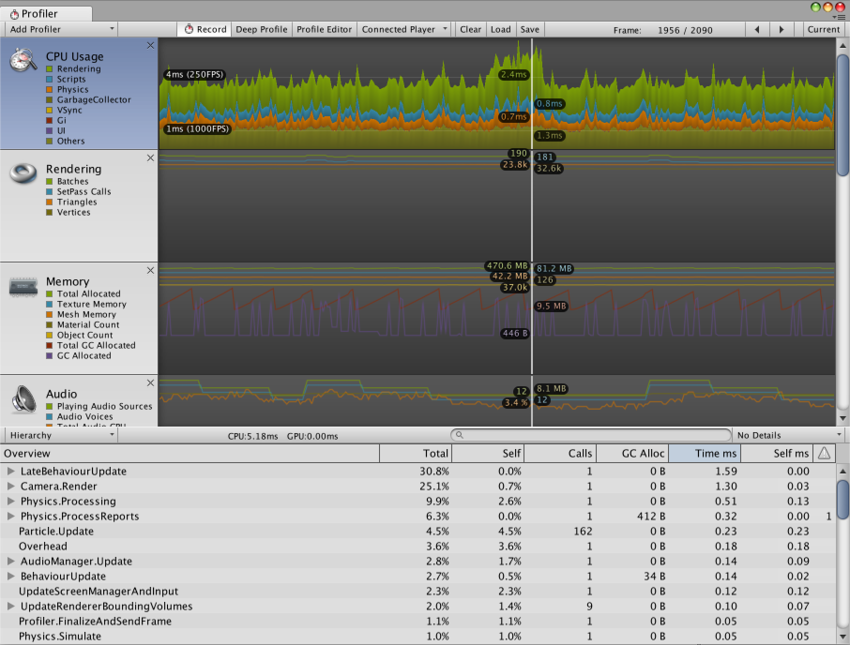
\includegraphics[width=1.0\textwidth,height=0.8\textheight]{UnityProfilerWindow}  
	\end{figure}
\end{frame}

\begin{frame}{Unity Profiler: Hints \& Tips}
	\begin{itemize}
		\pause \item You can remove items from the profiler graph by click on the colour box
		\pause \item Enabling \textbf{Deep Profile} will add a significant overhead to larger games
		\begin{itemize}
			\pause \item Surround you code with \textbf{Profiler.BeginSample} \& \textbf{Profiler.EndSample} this will appear in the Profiler
		\end{itemize}
		\pause \item You should consider Profiling a development build as the Editor adds significant overheard
	\end{itemize}
\end{frame}

\begin{frame}{Unreal Profiler}
	\begin{itemize}
		\pause \item The Unreal Profiler is built into the engine
		\pause \item It can accessed via \textbf{Window > Developer Tools > Session Frontend}
		\pause \item Allows us to profile all major systems
	\end{itemize}
\end{frame}

\begin{frame}{Unreal Profiler}
	\begin{figure}
		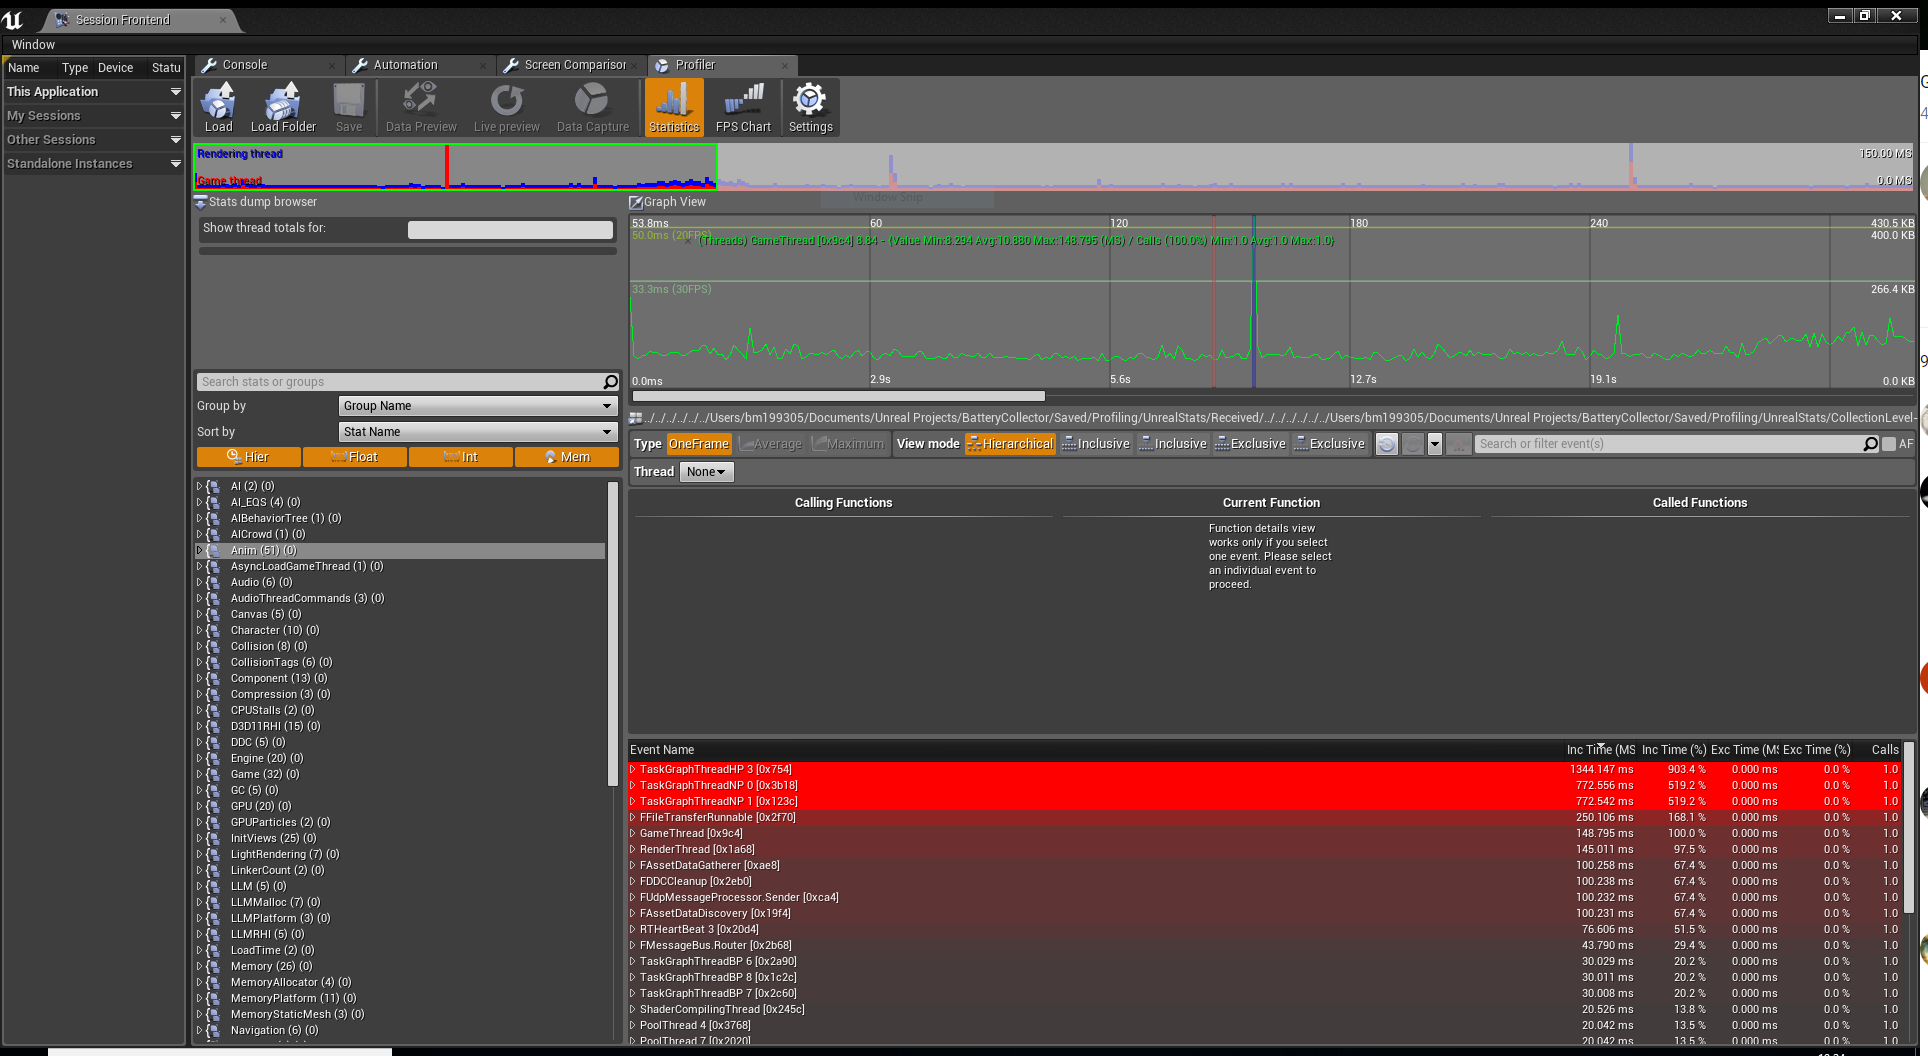
\includegraphics[width=1.0\textwidth,height=0.8\textheight]{UnrealProfilerWindow}  
	\end{figure}
\end{frame}
\part{Code smells}
\frame{\partpage}

\begin{frame}{Code smells}
    \begin{itemize}
        \pause\item ``Code smells'' are a useful guideline for refactoring
        \pause\item Warning signs that code needs to be refactored
        \pause\item \url{https://blog.codinghorror.com/code-smells/}
        \pause\item See also ``How to write unmaintainable code'' \url{https://github.com/Droogans/unmaintainable-code}
    \end{itemize}
\end{frame}



\end{document}
